\begin{homeworkProblem}
    \textbf{(2.16)} An impedance \( Z \) is built from a resistor and capacitor connected in parallel. When connected to an AC voltage source with a frequency of \( f = 60 Hz \), the impedance has a numerical value of \( Z = 1000(1 - j) \Omega \). The impedance is connected as shown in Figure 2.19, where the voltage source has an amplitude of \( 10V \) and at \( t = 0 \), the AC voltage is at a maximum.


\begin{figure}[H]
  \centering
  \includegraphics[width=0.45\textwidth]{../assets/H3P1F1.png}
\end{figure}

    \begin{enumerate}[(a)]
        \item What are the values of \( R \) and \( C \)? 
            \begin{callout}{Solution:}

                We have an equivalent impedance in the branch:
                \[ Z = 1000(1-j)~\Omega = \left( \frac{1}{R} + \frac{1}{\frac{1}{j \omega C}} \right)^{-1} \]
                Where $\omega = 2\pi f = 120\pi$. The real part is $R$ and the imaginary part is $Z_C$, giving the convenient relation:
                \begin{gather*}
                    R = 1000 \, \Omega \\ 
                    1000 = \frac{1}{\omega C}, \quad \Rightarrow \quad C = \frac{1}{1000 \omega} \, \text{C}
                \end{gather*}

            \end{callout}

            \newpage
        \item What is the power dissipated during one AC cycle in the impedance?
            \begin{callout}{Solution:}

                We have a definition of power dissipation given as:
                \[ P=I_{\text{rms}} V_{\text{rms}} \cos\phi = I^2 R \]
                \begin{align*}
                    i_{R}(t) &= \frac{V}{R} = \frac{10 \phase{0^\circ} }{1000} = 0.01 \phase{0^\circ} \textrm{~A} \\ 
                    i_{C}(t) &= \frac{V}{\frac{1}{j \omega C}} = j \omega CV = j(1000) \phase{90^\circ} \textrm{~A} \\ 
                    i(t) &= IR + IC = 0.01 \phase{0^\circ} + 0.01 \phase{90^\circ} = 0.01(1+j) \textrm{~A} \\
                    \operatorname{Re}(i(t)) &= 0.01(1+1)^{1 / 2} = 0.01 \sqrt{2} \textrm{~A}
                \end{align*}
                We then have power dissipated:
                $$P = I^2 R = (0.01)^2 \cdot 1000 = 0.1 \textrm{~W}$$

            \end{callout}

        \item What is the current in the resistor, \( i_R(t) \)?
           \begin{callout}{Solution:}

               Obtained in part (b)

           \end{callout}

        \item What is the current in the capacitor, \( i_C(t) \)?
           \begin{callout}{Solution:}

               Obtained in part (b)

           \end{callout}

        \item What fraction of the power from part (b) is dissipated in the resistor and the capacitor?
           \begin{callout}{Solution:}

           All power is dissipated in the resistor. Capacitors don't dissipate power.

           \end{callout}
    \end{enumerate}
\end{homeworkProblem}

\newpage
\begin{homeworkProblem}

    \begin{figure}[H]
        \centering
        \includegraphics[width=0.4\textwidth]{../assets/H3P2F1.png}
    \end{figure}

    \textbf{(2.18)} Figure 2.23 is an image of your oscilloscope from lab. The solid curve is channel 1 and the dashed curve is channel 2. You may assume that the input to your circuit is displayed on channel 1 and the output from your circuit is on channel 2. Answer the following questions based on these measured scope traces. 

    \begin{enumerate}[(a)]
        \item What is the frequency of the input signal? 
            \begin{callout}{Solution:}
                There is a period of 1 second, so there is also a frequency of 1 hz.
            \end{callout}
        \item What is the "peak-to-peak" and the "RMS" voltage of the output signal?  
            \begin{callout}{Solution:} 

                The it seems the waveform goes from -1.5 to 1.5 V, so the peak-to-peak is 3V. The RMS is, in general, given by the integral:
                $$ V_{\text{RMS}} = \sqrt{\frac{1}{T} \int_{0}^{T} V^2 \cos^2 (\omega t) \,dt} $$
                But for sinusoidal waveforms, it's simply
                $$ V_{\text{RMS}} = \frac{V_{\text{PK}}}{\sqrt{2}} $$
                So the RMS is $\tfrac{1.5}{\sqrt{2}}$.

            \end{callout}
        \item For this particular frequency, what is the gain, $|G|$, of your circuit? 

            \begin{callout}{Solution:}

                Gain is given as output/input amplitude, so we have 
                $$|G| = \frac{1.5}{4} = 0.375 = 20\log_{10}(0.375)\, \text{db} = -8.52\, \text{db}$$

           \end{callout}

        \item For this particular frequency, what is the phase difference
            $$ \Delta \phi=\phi_{o u t}-\phi_{\text {in }} $$
            (in degrees) between the input and output? 
           \begin{callout}{Solution:}

           Sinusoidal waveforms are of form:
               $$V(t) = \sin(\omega t + \phi) = \sin(2\pi f + \phi)$$
               Channel 1 is ahead of channel 2 by 0.2 seconds, and both have the same period of 1 second. 
               It follows that they have a frequency of 1 Hz as well. The angular frequency is then
               $2\pi$ rad / s. With the time difference, 
               $$ \boxed{\Delta \phi = 2\pi \cdot 0.2 = 0.4\pi\text{rad} = 72^\circ} $$

           \end{callout}
       \item Accurately sketch what the output signal would look like if the phase difference from part (d) were $180^{\circ}$.
           \begin{callout}{Solution:}

               \centering
               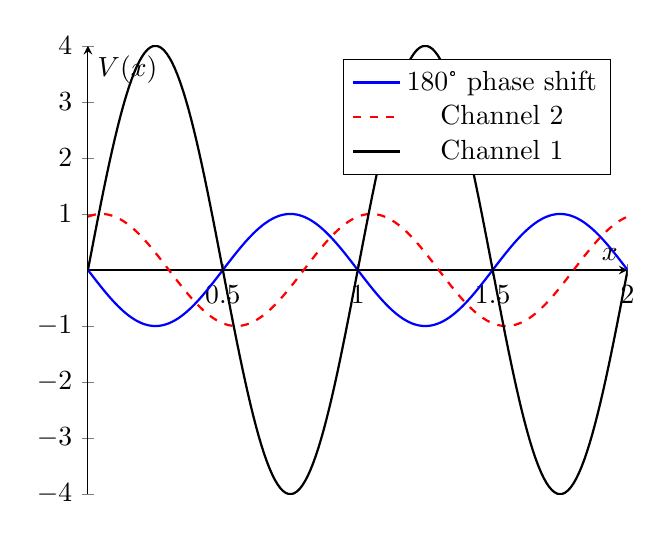
\begin{tikzpicture}
                   \begin{axis}[
                           axis lines = middle,
                           xlabel={$x$},
                           ylabel={$V(x)$},
                           samples=200,
                           domain=0:2,
                           legend pos=north east,
                           xtick={0,0.5,1,1.5,2},
                           ytick={-4,-3,-2,-1,0,1,2,3,4}
                       ]
                       % 180-degree phase shifted sine wave
                       \addplot[thick, solid, blue] {sin(deg(2*pi*x + pi))};
                       \addlegendentry{180° phase shift}

                       % Channel 2 (dashed line)
                       \addplot[thick, dashed, red] {sin(deg(2*pi*x + 0.4*pi))};
                       \addlegendentry{Channel 2}

                       % Channel 1 (amplified sine wave)
                       \addplot[thick, solid, black] {4*sin(deg(2*pi*x))};
                       \addlegendentry{Channel 1}

                   \end{axis}
\end{tikzpicture}

           \end{callout}
    \end{enumerate}

\end{homeworkProblem}

\begin{homeworkProblem}
    \textbf{(2.28)} If the curve on a Bode plot is falling off at \( 60 dB/\text{decade} \), what is the frequency dependence of the gain?
   \begin{callout}{Solution:}

   Each pole of a bode plot indicates that it is falling off of a gain of $-20$ dB / decade. The frequency dependence is 
       $$|G| \propto \frac{1}{f^3}$$
       where $f$ is the frequency, and $G$ is the gain.

   \end{callout}
\end{homeworkProblem}

\begin{homeworkProblem}
    LTSpice problem: Consider the circuit shown below (this is also the circuit for Part A of Experiment \#4). Use LTSpice to obtain plots of the power gain and phase shift as seen by the Ch. 2 output as a function of source frequency, with $10 \text{ Hz} \leq f_{\text{source}} \leq 10 \text{ kHz}$. Simulate a CR high-pass filter. Assume component values (C,R)=($10~\mu$F, 50$~\Omega$). (See video on "Bode plots with LTSpice.")

    \begin{figure}[H]
        \vspace{1em}
        \centering
        \begin{tabular}{|c|c|c|}
            \hline
            \( Z_1 \) & \( Z_2 \) & Type \\ 
            \hline
            L & R & low pass \\ 
            C & R & high pass \\ 
            R & C & low pass \\ 
            \hline
        \end{tabular}
    \end{figure}

    \begin{callout}{Solution:}

        \begin{enumerate}[(a)]
            \item LR Circuit (low-pass):
                \begin{figure}[H]
                    \centering
                    \begin{minipage}{0.49\textwidth}
                        \centering
                        \includegraphics[width=\textwidth]{../assets/H3P4F1.png}
                    \end{minipage}
                    \begin{minipage}{0.49\textwidth}
                        \centering
                        \includegraphics[width=\textwidth]{../code/p4-1.png}
                    \end{minipage}
                \end{figure}

            \item CR Circuit (high-pass):
                \begin{figure}[H]
                    \centering
                    \begin{minipage}{0.49\textwidth}
                        \centering
                        \includegraphics[width=\textwidth]{../assets/H3P4F2.png}
                    \end{minipage}
                    \begin{minipage}{0.49\textwidth}
                        \centering
                        \includegraphics[width=\textwidth]{../code/p4-2.png}
                    \end{minipage}
                \end{figure}

            \item RC Circuit (low-pass):
                \begin{figure}[H]
                    \centering
                    \begin{minipage}{0.49\textwidth}
                        \centering
                        \includegraphics[width=\textwidth]{../assets/H3P4F3.png}
                    \end{minipage}
                    \begin{minipage}{0.49\textwidth}
                        \centering
                        \includegraphics[width=\textwidth]{../code/p4-3.png}
                    \end{minipage}
                \end{figure}

        \end{enumerate}

    \end{callout}
\end{homeworkProblem}

\begin{homeworkProblem}
    LTSpice problem: Set up a series LRC circuit driven by an AC signal source. For this circuit, use $C = 10 ~\mu$F, $L = 10$ mH, and $R = 10 ~\Omega$. Generate a Bode plot of the power gain and a plot of the phase shift for $10 \text{ Hz} \leq f_{source} \leq 10 \text{ kHz}$. (See video on "Bode plots with LTSpice.") 
    \begin{callout}{Solution:}

        \begin{figure}[H]
            \centering
            \includegraphics[width=0.6\textwidth]{../assets/H3P5F1.png}
        \end{figure}

        \begin{figure}[H]
            \centering
            \includegraphics[width=0.6\textwidth]{../code/p5-1.png}
        \end{figure}

    \end{callout}
\end{homeworkProblem}

